% Reported held-out means and 95% Student-t intervals, five paired seeds.
% Provenance: ../../main.tex, Table tab:waterbirds-hidden-slice.
% Data are rounded published summaries, not reconstructed individual runs.
\documentclass[tikz,border=0pt]{standalone}
% Shared publication style. Compile figure sources from this directory.
\usepackage[T1]{fontenc}
\usepackage{lmodern}
\usepackage{amsmath,amssymb}
\usepackage{tikz}
\usepackage{pgfplots}
\usetikzlibrary{arrows.meta,calc,positioning,backgrounds,patterns,shapes.geometric}
\usepgfplotslibrary{groupplots,fillbetween}
\pgfplotsset{compat=1.18}
\definecolor{fgblue}{HTML}{0072B2}
\definecolor{fgorange}{HTML}{D55E00}
\definecolor{fgslate}{HTML}{8B949E}
\definecolor{fgdark}{HTML}{25313C}
\definecolor{fgpale}{HTML}{F2F6F8}
\definecolor{fggrid}{HTML}{E3E8EC}
\definecolor{fgwater}{HTML}{D6EAF4}
\definecolor{fgland}{HTML}{E8E3D3}
\renewcommand{\familydefault}{\sfdefault}
\tikzset{every picture/.style={font=\fontsize{9}{11}\selectfont,text=fgdark},
  panel label/.style={font=\bfseries\fontsize{10}{12}\selectfont,anchor=north west},
  panel title/.style={font=\bfseries\fontsize{9}{11}\selectfont,anchor=north west},
  light arrow/.style={-{Stealth[length=1.6mm]},draw=fgslate,line width=.65pt}}
\pgfplotsset{fg axis/.style={
  axis line style={fgslate,line width=.4pt},axis x line*=bottom,axis y line*=left,
  tick align=outside,tick style={fgslate,line width=.4pt},
  tick label style={font=\fontsize{8}{10}\selectfont,text=fgdark},
  label style={font=\fontsize{9}{11}\selectfont,text=fgdark},
  title style={font=\bfseries\fontsize{9}{11}\selectfont,text=fgdark},
  grid style={fggrid,line width=.35pt},minor tick num=0,
  legend style={draw=none,fill=none,font=\fontsize{8}{10}\selectfont},
  scaled ticks=false,clip=false,
  every axis plot/.append style={line width=.85pt,mark size=2.2pt}
}}

\begin{document}
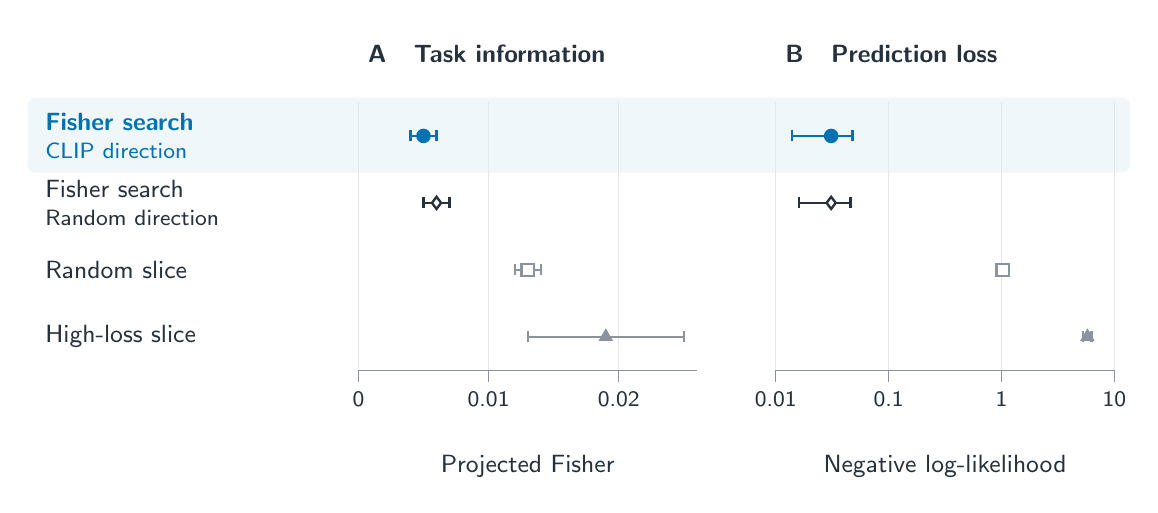
\begin{tikzpicture}[x=1mm,y=1mm]
\path[use as bounding box] (0,0) rectangle (140,58);
\fill[fgblue!6,rounded corners=1mm] (0,39.6) rectangle (140,49.1);
\node[panel title] at (42,57) {A\quad Task information};
\node[panel title] at (95,57) {B\quad Prediction loss};
\node[anchor=west,font=\bfseries\fontsize{9}{10.5}\selectfont,text=fgblue] at (1,46) {Fisher search};
\node[anchor=west,font=\fontsize{8}{10}\selectfont,text=fgblue] at (1,42.3) {CLIP direction};
\node[anchor=west] at (1,37.5) {Fisher search};
\node[anchor=west,font=\fontsize{8}{10}\selectfont] at (1,33.8) {Random direction};
\node[anchor=west] at (1,27.25) {Random slice};
\node[anchor=west] at (1,18.75) {High-loss slice};
\begin{axis}[fg axis,at={(42mm,14.5mm)},anchor=south west,
  width=43mm,height=34mm,scale only axis,
  xmin=0,xmax=.026,ymin=.5,ymax=4.5,
  axis y line=none,ytick=\empty,
  xtick={0,.01,.02},xticklabels={0,0.01,0.02},
  xmajorgrids=true,xlabel={Projected Fisher},
  xlabel style={at={(axis description cs:.5,-.28)},anchor=north},
  error bars/x dir=both,error bars/x explicit,
  error bars/error bar style={line width=.8pt},
  error bars/error mark options={rotate=90,mark size=2pt,line width=.8pt}]
\addplot+[only marks,fgblue,mark=*,mark options={fill=fgblue},error bars/.cd,x dir=both,x explicit]
 coordinates {(.005,4) +- (.001,0)};
\addplot+[only marks,fgdark,mark=diamond*,mark options={fill=white},error bars/.cd,x dir=both,x explicit]
 coordinates {(.006,3) +- (.001,0)};
\addplot+[only marks,fgslate,mark=square*,mark options={fill=white},error bars/.cd,x dir=both,x explicit]
 coordinates {(.013,2) +- (.001,0)};
\addplot+[only marks,fgslate,mark=triangle*,mark options={fill=fgslate},error bars/.cd,x dir=both,x explicit]
 coordinates {(.019,1) +- (.006,0)};
\end{axis}
\begin{axis}[fg axis,at={(95mm,14.5mm)},anchor=south west,
  width=43mm,height=34mm,scale only axis,
  xmode=log,log basis x=10,xmin=.01,xmax=10,ymin=.5,ymax=4.5,
  axis y line=none,ytick=\empty,
  xtick={.01,.1,1,10},xticklabels={0.01,0.1,1,10},
  xmajorgrids=true,xlabel={Negative log-likelihood},
  xlabel style={at={(axis description cs:.5,-.28)},anchor=north},
  error bars/error bar style={line width=.8pt},
  error bars/error mark options={rotate=90,mark size=2pt,line width=.8pt}]
\addplot+[only marks,fgblue,mark=*,mark options={fill=fgblue},error bars/.cd,x dir=both,x explicit]
 coordinates {(.031,4) +- (.017,0)};
\addplot+[only marks,fgdark,mark=diamond*,mark options={fill=white},error bars/.cd,x dir=both,x explicit]
 coordinates {(.031,3) +- (.015,0)};
\addplot+[only marks,fgslate,mark=square*,mark options={fill=white},error bars/.cd,x dir=both,x explicit]
 coordinates {(1.025,2) +- (.059,0)};
\addplot+[only marks,fgslate,mark=triangle*,mark options={fill=fgslate},error bars/.cd,x dir=both,x explicit]
 coordinates {(5.779,1) +- (.496,0)};
\end{axis}
\end{tikzpicture}
\end{document}
